\section{Large Organization Scenario}
\label{sec:large}

The evolving passwords scheme with location-based physical access controls can be deployed by a large organization in a big building with many visitors coming and leaving everyday. Considering a wide WLAN in a big building, there shall be several APs with their wireless signal covering the whole building. We assign one of such APs as the physical parameter generator and call it master AP. Physical parameters are broadcast though master AP’s wireless signal. By this way, mobile devices can only get physical parameters in the constrained location. Thus, only users who pass physical access controls and enter the constrained location can get physical parameters and synchronize their passwords with APs after passwords evolving. 	

\subsection{General Framework}
A WLAN system deployed with the proposed evolving passwords scheme consists of three parts: 
\begin{itemize}
    \item a master AP which can update its own password independently,
    \item several slave APs which can update their own passwords by interaction with the master AP, 
    \item many mobile devices which can connect to APs and automatically synchronize their own passwords with APs’.
\end{itemize}

The passwords evolving procedure can be divided into four: 
\begin{itemize}
    \item initial password setup and distribution,
    \item password update interval setup, 
    \item physical parameter generation and broadcast,
    \item password update of APs and mobile devices. 
\end{itemize}

The former two procedures will be executed only once in the initialization phase when the procedure starts, while the latter procedures will be repeatedly executed in the passwords evolving phase at regular intervals. 


In the initialization phrase, an initial password and an update interval is set by administrators and stored in configuration files on the master AP. An authenticator on the master AP reads the initial password and the update interval from configuration files when launched. For slave APs, it is unnecessary for administrators to set initial passwords for every slave AP. Instead, administrators specify the address of the master AP for slave APs, so authenticators on slave APs could acquire the current password from the master AP by a safe way. As for mobile devices,  initial passwords are obtained through an out-of-band way and the latest password will be stored in configuration files. 

After initialization, all APs will automatically update their passwords at regular intervals preset by administrators, while mobile devices will automatically synchronize their passwords with APs and join WLAN if possible. The evolving passwords phrase of every part is shown as graph 2. 

\begin{figure}
    \centering
    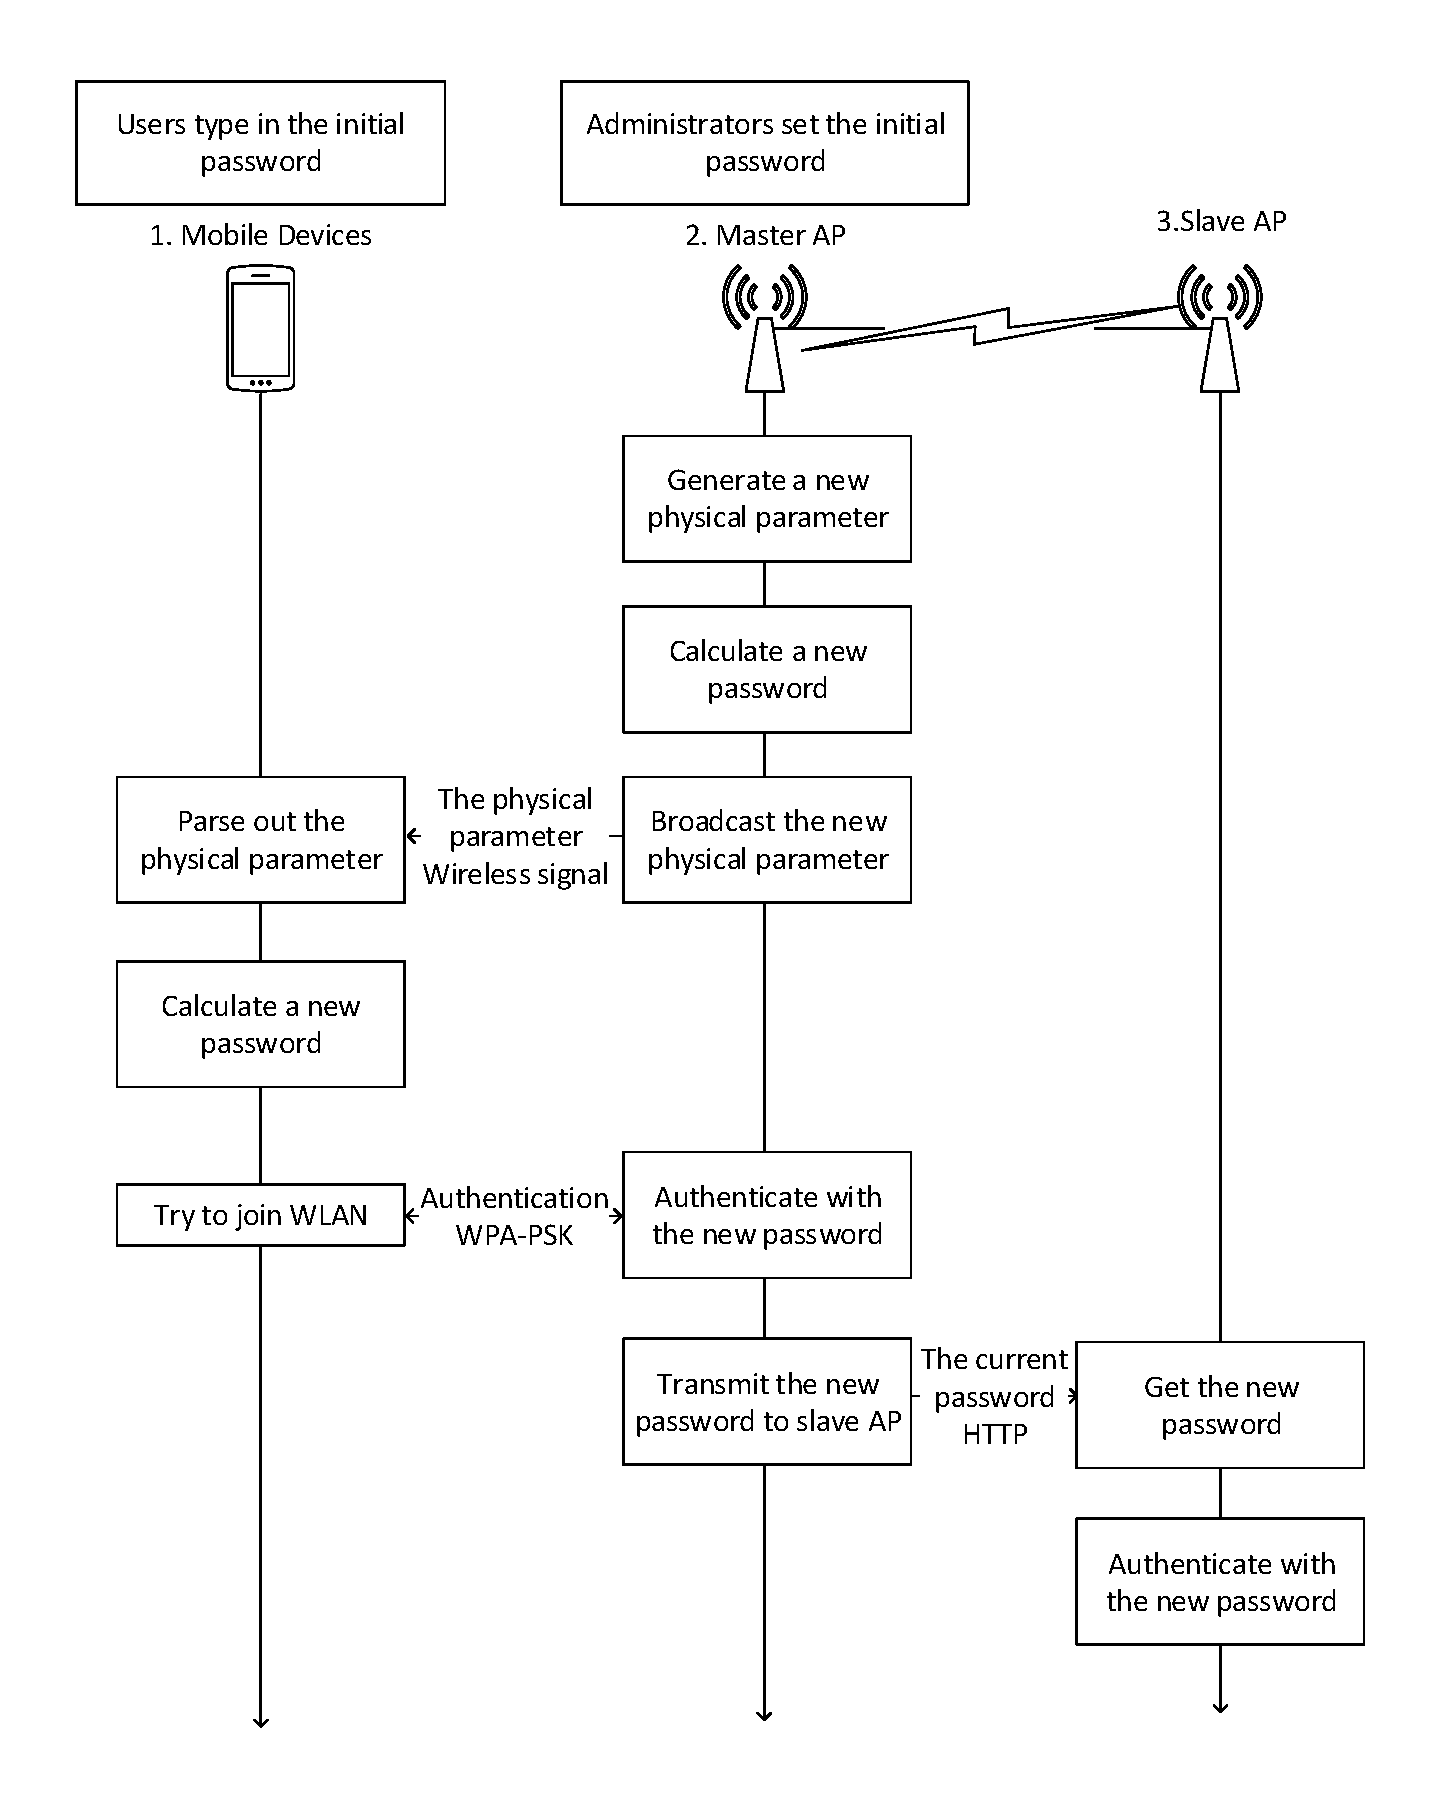
\includegraphics[width=0.5\textwidth]{pic/2.pdf}
    \caption{The Work Flow of the WLAN System with Location Related Dynamic Passwordd.}
    \label{fig:xxx}
\end{figure}


For the master AP, it need to complete the following works: 
\begin{itemize}
    \item Generate a long random number as a new physical parameter; 
    \item Calculate a new password using the old password and the new physical parameter; 
    \item Broadcast the new physical parameter to the constrained location protected by physical access controls; 
    \item Transmit the new password to slave APs securely. 
    \item Authenticate mobile devices using the new password; 
\end{itemize}
	

As for slave APs, they need to complete the following works: 
\begin{itemize}
    \item Require a new password from the master securely; 
    \item Authenticate mobile devices with the new password. 
\end{itemize}
	
As for mobile devices, they need to complete the following works: 
\begin{itemize}
    \item Capture WLAN signal and parse out the physical parameter from it; 
    \item Calculate out a new password by the same way with the master AP; 
    \item Try to join WLAN with the new password; 
    \item If joining successfully, accept the new password;
    \item If not, reject the new password and roll back.  After that, mobile devices can continuously join WLAN before next time passwords evolving. 
\end{itemize}

\subsection{Specific Detail}
The proposed evolving passwords system has some details which are worth specifying. 

\subsubsection{Password Format}
Mobile devices can join WLAN by the 802.11i protocol if they share the same pre-shared key with APs. In the 802.11i protocol, there are two password related concepts: passphrase and pre-shared key. The passphrase is a short string usually containing 8-20 characters which is easy to remember and type. Usually the passphrase is used to generate a 32 byte pre-shared key using a pseudo random generation algorithm. Then the pre-shared key will be used in a 4-way handshake for authentication between mobile devices and APs. 


In the proposed evolving passwords scheme, the password is the same as the pre-shared key with a length of 32 bytes which is the result of a secure hash algorithm such as SM3, SHA256. If the hash result is longer than 32 bytes,the first 32 byte of the result is used as the pre-shared key. The pre-shared key is too long to type in, we use the QR code to distribute it. The pre-shared key can be displayed on the screen or printed on the paper in the form of QR code. Authorized users can get the current password by scanning the QR code. As most of mobile devices are equipped with camera, it will not be a big problem for authorized users. 

\subsubsection{Password Update Interval}
In the initialization phrase, an update interval is set by administrators and it can be adjusted according to practical circumstances. In general, administrators can set a slightly longer update interval. However, when something important happens, they can shorten it for security considerations. This feature can be achieved as follows. 

All passwords have their expiry time, every time the master AP updates its password, its expiry time is increased by the the update interval. When slave APs require the current password, its expiry time will be responded at the same time. So slave APs know when the current password will be expired and when to request for a newer password from the master AP. 

If administrators want to change the update interval, he/she could modify the update interval and restart the authenticator on the master AP. When the authenticator restarts, it will continue using the current password until it is expired. However, when the current password is expired, the master AP will apply the new update interval. For slave APs, they get the expire time from the master AP, so modifying the update interval will not influence the update procedure of all APs in WLAN. 


However, if administrators do not want to wait until the current password expired, they have to modify the expiry time of the current password, and then restart all authenticators on the master AP and slave APs. By this way, the current password is forced to be expired in advance. 

\subsubsection{Broadcast Method of Physical} Parameters
At the process of the passwords evolving phrase, an physical parameter is generated and broadcast by the master AP. Physical parameters can be broadcast by the master AP’s wireless signal as it is limited in a constrained location. The beacon frame can be used to broadcast physical parameters. Usually, an AP will broadcast beacon frames at short intervals to announce existing of a special WLAN. There is a vendor specific field in the beacon frame which can carry custom data. The data structure of the vendor specific field consists of three parts: tag, length, and value. Custom data is carried in the value part. Different kinds of custom data is distinguished by the first 3 bytes called OUI. The next byte of OUI is OUI type. And the structure of the subsequent data depends on the concrete type of custom data, aka, OUI. The WLAN system can use a non-conflict OUI specially for physical parameter transmission. When mobile devices capture a beacon frame with a specific SSID, they can parse out the physical parameter in the vendor specific according to the predetermined OUI and OUI type. 

\subsubsection{Variable Broadcast Number of Physical Parameters} 
The master AP can broadcast one or more physical parameters to adjust the frequency of authorized users entering the constrained location. If the master AP update one password and broadcast one physical parameter , authorized users must enter the constrained location in every update period. If an authorized user has not entered the constrained location in one update period, he/she would never calculate out subsequent passwords. Even if he/she enters the constrained location in the next update period, he/she cannot calculate out the current password as he/she does not know the previous password which is necessary for calculating the current password. However, if the master AP broadcasts two physical parameters aka current and next physical parameter, it does not matter if an authorized user does not enter the constrained location in the next update period after he/she enters the constrained location in the current update period. Using the two physical parameters, he/she are able to calculate out the current and next password. When he/she enters the constrained location in the next of the next update period, he/she could still calculate out the password. If the master AP broadcasts more physical parameters, the time span authorized users entering the constrained location can be even longer. 


This feature can be applied to such a situation. Usually, the staff is required to be on duty every weekday. So the update interval can be set to one day. However, the staff may not go to work at the weekend. If the master AP still broadcasts one physical parameter on Friday, the staff cannot join WLAN on Monday. For the staff successfully joining WLAN on Monday, the master AP should generates and broadcasts three physical parameters on Friday. 

\subsubsection{Passwords Evolving Formula}
Once the master AP generates a new physical parameter, it calculates a new password with the old password and the new physical parameter. Let P[i - 1] as the old password, O[i] as the new physical parameter, the new password P[i] can be calculated out as follows: 
P[i] = Truncate(Hash(P[i - 1] XOR O[i]))\cite{m2005hotp}\cite{Liu2014An}. 
The hash algorithm can be SM2, SHA-256, and the like. As mentioned above, the password is a 32 byte number, but the hash value may be longer than 32 bytes. In this case, we can truncate the first 32 bytes of the hash value as the new password. 



\subsubsection{Password Transmission Channel between the Master AP and Slave APs} 
In the initialization phrase, slave APs should request for the initial password from the master AP. When the current password is expired, slave APs should request for a new password from the master AP. The password should be transmitted from the master AP to slave APs though a secure channel. For example, administrators can establish dedicated links for transmitting passwords between the master AP and slave APs. For another example, the above information can be transmitted through a common LAN. Though such LAN is insecure as it is connected with WLAN and Internet, the master AP can secure it by encrypting and adding a message authentication code before transmitting passwords, ensuring that only the master AP and slave APs share secret keys. It is also a proper way to establish a mutual authenticated TLS tunnel between the master AP and slave APs on LAN and transmit passwords in the TLS tunnel. 


\subsubsection{Password Synchronization between the Master AP and Slave APs}
The system time of slave APs may be later than that of the master AP. If so, there may be an out of sync of password update between the master AP and slave APs. That is, the master AP has updated passwords, but slave APs still use old passwords as it thinks old passwords have not been expired yet. To achieve a near-zero time delay between the master AP and slave APs, all APs should regularly adjust the system time from the same time server. Besides, slave APs could request a new password slightly earlier than the expiry time of the current password. If there is a long time delay between an slave AP and the master AP, mobile devices may not be able to connect to slave APs when they have once received a beacon frame from the master AP and already updated their own passwords. 



\subsubsection{Passwords Synchronization between APs and Mobile Devices}
If all APs update their own passwords, only mobile devices update their own passwords synchronously could they join WLAN again. Considering the update interval can be adjusted by administrators on demand, it becomes a problem how to inform mobile devices whether passwords evolve and how many times passwords have been evolved from mobile devices getting their initial passwords or updating their passwords last time. To solve this problem, we assign a serial number for the password. The serial number starts with zero and increases by one after passwords evolving. APs broadcast the serial number of the password they currently use to inform mobile devices whether they need to update their own passwords. Serial numbers can be broadcast through the beacon frame using the vendor specific field like physical parameters. They can have the same OUI but different OUI type compared with physical numbers. 


When mobile devices get the current password from administrators or other authorized users, its serial number is same. Mobile devices regularly capture and parse beacon frames. Once capturing frames with a specific SSID, mobile devices will parse out the serial number, and determines whether they share the same password with APs by comparing the two serial numbers. If the serial numbers of APs’ passwords is the same as that of their own passwords, it means they share the same password with APs and can join WLAN using the old passwords. If the serial number of APs’ passwords is greater by one than that of their own passwords, mobile devices can update their own passwords if they can get the current physical parameter. If else, mobile devices cannot update their own passwords to the current time. The system time of APs and mobile devices may also be different. However, it is not a big deal. Mobile devices use the serial number to determine whether they can synchronize their passwords with APs. The system time of mobile devices does not participate in the password update process. 


\subsubsection{Verification of Physical Parameters by Mobile Devices}
If mobile devices successfully parse out a physical parameters from a beacon frame, they calculate a temporary new password without updating their own passwords because the physical parameter may be wrong. Then it tries to join WLAN using the temporary new password. If it successfully connect to APs, it means the temporary new password is right. Until then, mobile devices could update their own passwords. If mobile devices fail to connect to APs, they should clear the temporary new password and wait for another physical parameter. 


\subsubsection{Consideration of an Unexpected or Planned Restart}
Once calculating out a new password, the master AP should store the new physical parameter and the new password with its expiry time into configuration files in case of an unexpected or planned restart. By this way, even if the master AP experiences an unexpected or planned restart, it still could get the newest physical parameter and the newest password. Therefore, it could continue broadcasting the newest physical parameter, use the newest password to authenticate mobile devices.


When the master AP restarts, the password in configuration files may have been expired. The master AP determines whether such password is expired by getting the current time and comparing it with the expiry time of the password. If the current time exceed the expiry time of the password, it should update the password to the current time. 


Mobile devices have a similar situation with the master AP, and they should also update configuration files when their passwords are updated. However, An unexpected or planned restart will not influence slave APs because they get the newest password from the master AP when they start. 

